\documentclass{jthesis}

\usepackage{amsfonts}
\usepackage{amsmath}
\usepackage{geometry}
\usepackage{amsthm}
\usepackage{mathrsfs}
\usepackage{setspace}
\usepackage{footmisc}
\usepackage{hyperref}
\usepackage{xcolor,graphicx}
\usepackage{subcaption}
\usepackage{amssymb}

\title{Collisions of Primordial Black Holes with Neutron Stars} %Don't put a line break in, it gets really upset
\author{Brady Metherall}
\date{March 30, 2017}

\setlength\parindent{0pt}

\DeclareMathOperator{\sgn}{sgn}
\DeclareMathOperator{\Heavi}{H}

\DeclareMathOperator{\Hsign}{\mathscr{H}}
\newcommand\Hank[2][]{{\left( \Hsign_{#1} #2 \right) }}

\DeclareMathOperator{\grad}{\overset{\rightharpoonup}\nabla}

\newtheorem{theorem}{Theorem}[chapter]
\newtheorem{definition}[theorem]{Definition}
\newtheorem{corollary}[theorem]{Corollary}
\newtheorem{lemma}[theorem]{Lemma}

\renewcommand{\thefootnote}{\fnsymbol{footnote}}

\begin{document}

\pagenumbering{roman}
\maketitle

\makeabstract{
This is a short example of an abstract.
}

\makeacknowledgements{
Thank some people that you like here.
}

\makedeclaration

\maketableofcontents

\pagenumbering{arabic}
\doublespacing
\linespread{2}


%\documentclass[12pt]{article}
%
%\usepackage{amsfonts}
%\usepackage{amsmath}
%\usepackage{geometry}
%\usepackage{amsthm}
%\usepackage{mathrsfs}
%\usepackage{setspace}
%\usepackage{footmisc}
%
%\newgeometry{margin=1in}
%\setlength\parindent{0pt}
%
%\DeclareMathOperator{\sgn}{sgn}
%\DeclareMathOperator{\Heavi}{H}
%
%\DeclareMathOperator{\Hsign}{\mathscr{H}}
%\newcommand\Hank[2][]{{\left( \Hsign_{#1} #2 \right) }}
%
%\newtheorem{theorem}{Theorem}[section]
%\newtheorem{definition}[theorem]{Definition}
%\newtheorem{corollary}[theorem]{Corollary}
%\newtheorem{lemma}[theorem]{Lemma}
%
%\renewcommand{\thefootnote}{\fnsymbol{footnote}}
%
%\begin{document}
%
%\doublespacing
%\linespread{2}

\chapter{Operators and Integral \\ Transforms}
\label{chap:hank}

Before starting the in-depth analysis, we first must introduce key definitions, and theorems, several of which have been modified from \cite{functional}, to more easily analytically solve the velocity potential of the neutron star.

\begin{definition}[Operator]
\label{def:operator}
Let $A$, and $B$ be vector spaces with respective subspaces, $X$, and $Y$. An operator $\mathcal{T}$, maps any $x \in X$ to $Y$, and is denoted by $\mathcal{T}(x)$.
\end{definition}

Common examples of operators are the Sturm-Liouville operator, the Laplacian, or the Hamiltonian. Our focus will be on the integral operator, or transform.

\begin{definition}[Integral Transform]
\label{def:transform}
Let the domain, and co-domain of the transform be $C[a,b]\footnote[4]{$C[a,b]$ denotes the set of continuous functions on the interval $[a,b]$. Likewise, $C^n[a,b]$ denotes the set of functions whose $n$-th derivative is continuous on the interval $[a,b]$.}$ and $K: \mathbb{R}^2 \rightarrow \mathbb{R}$, then we can define our operator $\mathcal{T}:C[a,b] \rightarrow C[a,b]$ as
\begin{align*}
(\mathcal{T}f)(x) = \int_a^b f(y) K(x,y) \, dy,
\end{align*}
where $K$ is called the kernel function.
\end{definition}

During the analysis, a specific integral transform will be used, namely the Hankel transform, which will be defined shortly. Typically, the bounds of integral transforms are either $0$ or $-\infty$, to $\infty$, and therefore, the following definition and theorem are necessary to show that integral transforms are well behaved, and continuous.

\begin{definition}[Uniform Continuity]
A function $f: X \rightarrow Y$, with $X, \, Y \subseteq \mathbb{R}$, is uniformly continuous if $\forall \varepsilon > 0$, $\exists \, \delta > 0 \, : \, |x-x_0| < \delta \Rightarrow |f(x) - f(x_0)| < \varepsilon$, $ \forall x_0 \in X$.
\end{definition}

Uniform continuity has a very similar formal definition to continuity, the difference being of course, is that  $\delta$ must be the same for the entire domain. Furthermore, continuity is only defined for a point, whereas uniform continuity is defined over an interval.

\begin{theorem}[Heine-Cantor Theorem]
% http://projecteuclid.org/download/pdf_1/euclid.acta/1485881938
% page 23 theorem 1
If a function $f: X \rightarrow \mathbb{R}$, with $X$ a closed, subset of the real numbers, is continuous, $f$ is uniformly continuous on $X$.
\label{thm:uniform}
\end{theorem}
\begin{proof}
Since $f$ is continuous, by Cousin's Theorem \cite{cousin} there exists a finite subcover of $X$\footnote[4]{Figure \ref{fig:arrows} helps visualize the concept of finite subcovers.}:
\begin{align*}
\{ B_{\delta_i/2} (x_i) : 1 \leq i \leq n \in \mathbb{N} \} : X \subseteq \bigcup_{i=1}^n B_{\delta_i/2}(x_i),
\end{align*}
such that
\begin{align*}
\forall \, \frac{1}{2}\varepsilon > 0, \, \exists \, i : |x-x_i| < \frac{1}{2} \delta_i \Rightarrow |f(x)-f(x_i)| < \frac{1}{2}\varepsilon \, \forall \, x \in X.
\end{align*}
Now, let $\delta = \min \{ \frac{1}{2} \delta_i : 1 \leq i \leq n \}$, and suppose, $|x-x_0| < \delta$, then, $\exists i : |x-x_i| < \frac{1}{2}\delta_i$.  Then,
\begin{align*}
|x_0-x_i| \leq |x_0-x| &+ |x-x_i| < \delta + \frac{1}{2}\delta_i \leq \delta_i, \\
|f(x_0)-f(x)| \leq |f(x_0)-f(x_i)| &+ |f(x_i)-f(x)| < \frac{1}{2}\varepsilon + \frac{1}{2}\varepsilon = \varepsilon
\end{align*}
by the triangle inequality.
\end{proof}

\begin{figure}[!p]
\centering
% GNUPLOT: LaTeX picture with Postscript
\begingroup
  \makeatletter
  \providecommand\color[2][]{%
    \GenericError{(gnuplot) \space\space\space\@spaces}{%
      Package color not loaded in conjunction with
      terminal option `colourtext'%
    }{See the gnuplot documentation for explanation.%
    }{Either use 'blacktext' in gnuplot or load the package
      color.sty in LaTeX.}%
    \renewcommand\color[2][]{}%
  }%
  \providecommand\includegraphics[2][]{%
    \GenericError{(gnuplot) \space\space\space\@spaces}{%
      Package graphicx or graphics not loaded%
    }{See the gnuplot documentation for explanation.%
    }{The gnuplot epslatex terminal needs graphicx.sty or graphics.sty.}%
    \renewcommand\includegraphics[2][]{}%
  }%
  \providecommand\rotatebox[2]{#2}%
  \@ifundefined{ifGPcolor}{%
    \newif\ifGPcolor
    \GPcolorfalse
  }{}%
  \@ifundefined{ifGPblacktext}{%
    \newif\ifGPblacktext
    \GPblacktexttrue
  }{}%
  % define a \g@addto@macro without @ in the name:
  \let\gplgaddtomacro\g@addto@macro
  % define empty templates for all commands taking text:
  \gdef\gplbacktext{}%
  \gdef\gplfronttext{}%
  \makeatother
  \ifGPblacktext
    % no textcolor at all
    \def\colorrgb#1{}%
    \def\colorgray#1{}%
  \else
    % gray or color?
    \ifGPcolor
      \def\colorrgb#1{\color[rgb]{#1}}%
      \def\colorgray#1{\color[gray]{#1}}%
      \expandafter\def\csname LTw\endcsname{\color{white}}%
      \expandafter\def\csname LTb\endcsname{\color{black}}%
      \expandafter\def\csname LTa\endcsname{\color{black}}%
      \expandafter\def\csname LT0\endcsname{\color[rgb]{1,0,0}}%
      \expandafter\def\csname LT1\endcsname{\color[rgb]{0,1,0}}%
      \expandafter\def\csname LT2\endcsname{\color[rgb]{0,0,1}}%
      \expandafter\def\csname LT3\endcsname{\color[rgb]{1,0,1}}%
      \expandafter\def\csname LT4\endcsname{\color[rgb]{0,1,1}}%
      \expandafter\def\csname LT5\endcsname{\color[rgb]{1,1,0}}%
      \expandafter\def\csname LT6\endcsname{\color[rgb]{0,0,0}}%
      \expandafter\def\csname LT7\endcsname{\color[rgb]{1,0.3,0}}%
      \expandafter\def\csname LT8\endcsname{\color[rgb]{0.5,0.5,0.5}}%
    \else
      % gray
      \def\colorrgb#1{\color{black}}%
      \def\colorgray#1{\color[gray]{#1}}%
      \expandafter\def\csname LTw\endcsname{\color{white}}%
      \expandafter\def\csname LTb\endcsname{\color{black}}%
      \expandafter\def\csname LTa\endcsname{\color{black}}%
      \expandafter\def\csname LT0\endcsname{\color{black}}%
      \expandafter\def\csname LT1\endcsname{\color{black}}%
      \expandafter\def\csname LT2\endcsname{\color{black}}%
      \expandafter\def\csname LT3\endcsname{\color{black}}%
      \expandafter\def\csname LT4\endcsname{\color{black}}%
      \expandafter\def\csname LT5\endcsname{\color{black}}%
      \expandafter\def\csname LT6\endcsname{\color{black}}%
      \expandafter\def\csname LT7\endcsname{\color{black}}%
      \expandafter\def\csname LT8\endcsname{\color{black}}%
    \fi
  \fi
    \setlength{\unitlength}{0.0500bp}%
    \ifx\gptboxheight\undefined%
      \newlength{\gptboxheight}%
      \newlength{\gptboxwidth}%
      \newsavebox{\gptboxtext}%
    \fi%
    \setlength{\fboxrule}{0.5pt}%
    \setlength{\fboxsep}{1pt}%
\begin{picture}(7200.00,5040.00)%
    \gplgaddtomacro\gplbacktext{%
      \csname LTb\endcsname%
      \put(330,220){\makebox(0,0){\strut{}$1$}}%
      \put(1625,220){\makebox(0,0){\strut{}$1.2$}}%
      \put(2919,220){\makebox(0,0){\strut{}$1.4$}}%
      \put(4214,220){\makebox(0,0){\strut{}$1.6$}}%
      \put(5508,220){\makebox(0,0){\strut{}$1.8$}}%
      \put(6803,220){\makebox(0,0){\strut{}$2$}}%
      \put(524,3041){\makebox(0,0)[l]{\strut{}$\delta_1/2$}}%
      \put(1625,3041){\makebox(0,0)[l]{\strut{}$\delta_2/2$}}%
      \put(2919,3041){\makebox(0,0)[l]{\strut{}$\delta_3/2$}}%
      \put(4408,3171){\makebox(0,0)[l]{\strut{}$\delta_4/2$}}%
      \put(5120,3041){\makebox(0,0)[l]{\strut{}$\delta_5/2$}}%
      \put(5962,3041){\makebox(0,0)[l]{\strut{}$\delta_6/2$}}%
    }%
    \gplgaddtomacro\gplfronttext{%
    }%
    \gplbacktext
    \put(0,0){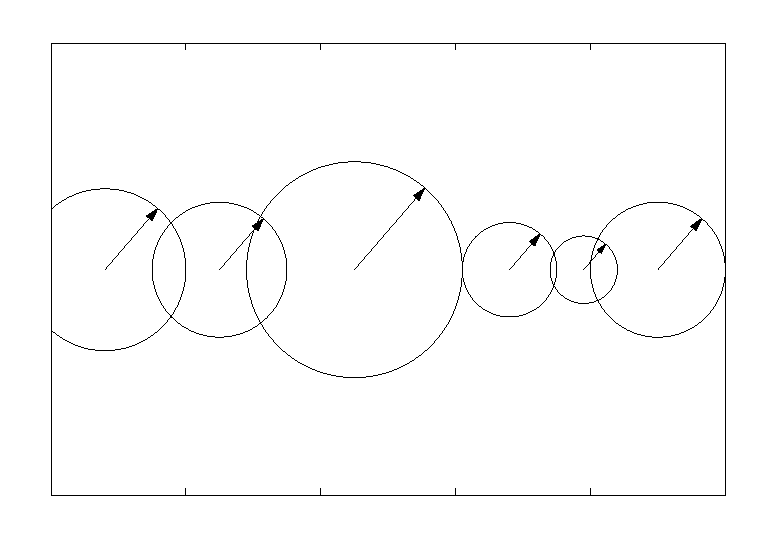
\includegraphics{Arrows}}%
    \gplfronttext
  \end{picture}%
\endgroup

\caption[Cousin's Theorem Depiction]{Cousin's Theorem states that there exists a finite subcover of a closed interval. For example, consider the interval $[1,2] \in \mathbb{R}$, then there exists a finite collection of circles (or more generally balls) of radii $\delta_i/2$ which spans the interval.}
\label{fig:arrows}
\end{figure}

Physically, we require the velocity potential to be continuous, and so the Hankel transform (and in fact all integral transforms) should preserve continuity, as shown in Theorem \ref{thm:continuity}.

\begin{theorem}
\label{thm:continuity}
$\mathcal{T}f$ is continuous if $\int_a^b |f(y)| dy < \infty$, and $K(x,y)$ is uniformly continuous on $[a,b]$.
\end{theorem}
\begin{proof}
For all $\varepsilon > 0$, choose $\delta : |x - x_0| < \delta$, so that $|K(x,y) - K(x_0,y)| < \varepsilon/M$, with $M = \int_a^b |f(y)| dy$. Then,
\begin{align*}
|(\mathcal{T}f)(x) - (\mathcal{T}f)(x_0)| &= \left| \int_a^b K(x,y)f(y) dy - \int_a^b K(x_0,y)f(y) dy \right| \\
&\leq \int_a^b |K(x,y) - K(x_0,y)||f(y)| dy \\
&< \int_a^b \frac{\varepsilon}{M} |f(y)| dy \\
&< \varepsilon,
\end{align*}
and $\mathcal{T}f$ is continuous.
\end{proof}

The conditions for Theorem \ref{thm:continuity} are automatically satisfied by Theorem \ref{thm:uniform} if $a$ and $b$ are finite, and $K$ is bounded and continuous.

\section{Hankel Transform}

The Hankel transform, named after the German mathematician Hermann Hankel, is quite common in cylindrically symmetric systems, such as ours, and arises from the eigenfunctions of Laplace's equation.

\begin{definition}[Hankel Transform]
\label{def:hanktrans}
The Hankel transform of a function $f(s)$ is given by
\begin{align*}
\Hank[\nu]{f}(\sigma) = \int_0^\infty f(s) J_\nu(s \sigma) s \, ds,
\end{align*}
where $J_\nu$ is the Bessel function of the first kind, of order $\nu \geq -\frac{1}{2}$, and $\sigma$ is a non-negative real variable.
\end{definition}

Notice too, that it directly follows from Definition \ref{def:hanktrans} that the Hankel transform is self-reciprocal.

\begin{corollary}[Inverse Hankel Transform]
\label{def:invhanktrans}
The Hankel transform is self-reciprocal, that is, the inverse Hankel transform is also given by Definition \ref{def:hanktrans}.
\end{corollary}
\begin{proof}
The Hankel transform is self-reciprocal
\begin{align*}
\iff f(s) &= \int_0^\infty \Hank[\nu]{f}(\sigma) J_\nu(s \sigma) \sigma \, d\sigma \\
\iff &= \int_0^\infty \int_0^\infty f(s') J_\nu(s \sigma) s' \, ds' J_\nu(s \sigma) \sigma \, d\sigma \\
&= \int_0^\infty f(s') s' \int_0^\infty J_\nu(s' \sigma) J_\nu(s \sigma) \sigma \, d\sigma \, ds' \\
&= f(s),
\end{align*}
by the orthogonality of the Bessel functions.
\end{proof}

However, only the order zero Hankel transform will be used in the analysis, so the $\nu$ shall be omitted and assumed zero, unless otherwise stated. Note that the kernel function of the Hankel transform is not $J_0 (s \sigma) s$, but in fact $\sqrt{s} J_0 (s \sigma)$, the other $\sqrt{s}$ factor gets absorbed into $f$. This is to ensure uniform continuity of the kernel (Lemma \ref{lem:Jcont}), and the continuity of the transform, while minimizing the constraint on $f$. As a consequence, we have the modified condition that $\int_0^\infty \sqrt{s}|f(s)| ds < \infty$.

\begin{lemma}
$\sqrt{s}J_0(s \sigma)$ is uniformly continuous on $[0,\infty)$.
\label{lem:Jcont}
\end{lemma}
\begin{proof}
Let $N$ be a sufficiently large number. By Theorem \ref{thm:uniform}, $\sqrt{s}J_0(s \sigma)$ is uniformly continuous on $[0,N]$. And on the interval $(N,\infty)$,
\begin{align*}
J_0(s \sigma) \rightarrow \sqrt{\frac{2}{\pi s \sigma}} \cos \left( s \sigma - \frac{\pi}{4} \right)
\end{align*}
asymptotically, and therefore $\sqrt{s}J_0(s \sigma)$ is uniformly continuous on $[0,\infty)$ since cosine is uniformly continuous everywhere by its periodicity.
\end{proof}

\begin{theorem}
The Hankel transform is continuous if $\int_0^\infty \sqrt{s}|f(s)| ds < \infty$.
\end{theorem}
\begin{proof}
Lemma \ref{lem:Jcont} shows the uniform continuity of the kernel, and $\int_0^\infty \sqrt{s}|f(s)| ds < \infty$ is a stronger condition than $\int_0^\infty |f(s)| ds < \infty$, thus by Theorem \ref{thm:continuity}, the Hankel transform is continuous.
\end{proof}

The following, and final theorem will be particularly useful for calculating the energy deposited to the neutron star.
\begin{theorem}
\label{thm:square}
The integral of the square of the Hankel transform weighted by $\sigma$ is equivalent to the integral of the square of the function weighted by $s$:
\begin{align*}
\int_0^\infty \Hank[\nu]{f}^2(\sigma) \sigma \, d\sigma = \int_0^\infty f^2(s)s \, ds.
\end{align*}
\end{theorem}

\begin{proof}
From the definition of the Hankel transform we have
\begin{align*}
\int_0^\infty \Hank[\nu]{f}^2(\sigma) \sigma \, d\sigma &= \int_0^\infty \int_0^\infty f(s) J_\nu(s \sigma) s \, ds \int_0^\infty f(s') J_\nu(s' \sigma) s' \, ds' \, \sigma \, d\sigma, \\
&= \int_0^\infty \int_0^\infty f(s) f(s') s \, s' \int_0^\infty J_\nu(s \sigma) J_\nu(s' \sigma) \sigma \, d\sigma \, ds \, ds', \\
&= \int_0^\infty f^2(s) s \, ds
\end{align*}
by the orthogonality of Bessel functions.
\end{proof}

\subsection{Applications of the Hankel Transform}

As previously noted, the Hankel transform arises from axisymmetric problems in cylindrical coordinates from the radial eigenfunction of Laplace's equation. Because of this, the Hankel transform along with the Laplace transform have many applications in solving partial differential equations in physics. Some examples include, but are not limited to, the free vibration of a circular membrane, the diffusion equation, acoustic radiation, or even the axisymmetric Cauchy-Poisson wave problem which shares many similarities with this work \cite{transforms}.

%\end{document}


%\documentclass[12pt]{report}
%
%\usepackage{amsfonts}
%\usepackage{amsmath}
%\usepackage{geometry}
%\usepackage{amsthm}
%\usepackage{mathrsfs}
%\usepackage{xcolor,graphicx}
%\usepackage{subcaption}
%\usepackage{setspace}
%\usepackage{amssymb}
%\usepackage{footmisc}
%
%\newgeometry{margin=1in}
%\setlength\parindent{0pt}
%
%\DeclareMathOperator{\sgn}{sgn}
%\DeclareMathOperator{\Heavi}{H}
%\DeclareMathOperator{\grad}{\overset{\rightharpoonup}\nabla}
%
%\DeclareMathOperator{\Hsign}{\mathscr{H}}
%\newcommand\Hank[2][]{{\left( \Hsign_{#1} #2 \right) }}
%
%\newtheorem{theorem}{Theorem}[section]
%\newtheorem{definition}[theorem]{Definition}
%\newtheorem{corollary}[theorem]{Corollary}
%
%\renewcommand{\thefootnote}{\fnsymbol{footnote}}
%
%\begin{document}
%
%\doublespacing
%\linespread{2}

\chapter{Analytic Solution}

Typically, in fluid dynamics, the scalar function known as the velocity potential denoted by $\varphi$, is the desired quantity. Once the velocity potential is known, the system is essentially solved because  $\grad \varphi = \overset{\rightharpoonup}u$, and in the case of a free surface, the deformation of the surface can readily be found from the velocity potential as well. The velocity potential will be found in the coming sections, along with the profile of the surface, and lastly the energy deposited into the neutron star will be calculated.

\section{Eigenfunctions of the Laplacian}

The first step in analytically solving for the velocity potential will be to find the eigenfunctions of Laplace's equation, $\nabla^2 \varphi = 0$, since the velocity potential is conservative. Since this is a partial differential equation we will assume the solution is the product of univariate functions, $\varphi = f(r) g(\theta) h(z) T(t)$. Expanding the Laplacian for cylindrical systems gives 
\begin{align*}
\frac{1}{r}\frac{\partial}{\partial r} \left( r \frac{\partial \varphi}{\partial r} \right) + \frac{1}{r^2} \left( \frac{\partial^2 \varphi}{\partial \theta^2} \right) + \frac{\partial^2 \varphi}{\partial z^2} = 0.
\end{align*}

The temporal component can be divided out since the Laplacian does not involve time, and will be found later on. Substituting in our assumed form, and dividing by $\varphi$, yields
\begin{align}
\label{eq:laplaciansub}
\frac{1}{fr}\frac{\partial}{\partial r}(rf') + \frac{1}{r^2}\frac{g''}{g} + \frac{h''}{h} = 0,
\end{align}

where primes denote the derivative with respect to the function's only variable. Notice that the function $h(z)$ has been separated from both $f(r)$, and $g(\theta)$, and since each function is univariate, it must be the case that the last term is constant --
\begin{align*}
\frac{h''}{h} = k^2.
\end{align*}

We cleverly force this constant to be positive to satisfy the boundary conditions, namely, that $h(-\infty) = 0$. The most general solution to this is of course exponentials --
\begin{align*}
h(z) = Ae^{kz} + Be^{-kz}.
\end{align*}

Since the velocity potential has to vanish at negative infinity, this is simplified to
\begin{align}
\label{eq:h}
h(z) = e^{kz},
\end{align}

without loss of generality we can assume the constant is one since it can be absorbed into $T(t)$. By substituting in $k^2$ and multiplying through by $r^2$, \eqref{eq:laplaciansub} becomes
\begin{align}
\label{eq:laplacenoh}
\frac{r}{f}\frac{\partial}{\partial r} \left( rf' \right) + k^2r^2 + \frac{g''}{g} = 0,
\end{align}

and once again, $g(\theta)$ has been separated from $f(r)$, and so the last term must be constant --
\begin{align*}
\frac{g''}{g} = -\mu^2.
\end{align*}

The constant is forced to be negative since $g(\theta)$ is expected to be periodic and not exponential. Of course, the general solution to this differential equation is 
\begin{align*}
g(\theta) = A \sin(\mu \theta) + B \cos(\mu \theta).
\end{align*}

However, our system is cylindrically symmetric; there is no way to differentiate one value of $\theta$ to another, thus, it is expected that $\varphi$ has no $\theta$ dependence, and consequentially, $g(\theta)$ must be constant, the only way this is satisfied is if $\mu = 0$, so that
\begin{align}
\label{eq:g}
g(\theta) = 1.
\end{align}

By substituting $\mu = 0$ into \eqref{eq:laplacenoh}, and multiplying through by $f$ we obtain
\begin{align*}
r \frac{\partial}{\partial r}(rf') + (k^2r^2 - 0^2)f = 0,
\end{align*}

which is indeed Bessel's differential equation of order $0$. Therefore,
\begin{align*}
f(r) = A J_0(kr) + B Y_0(kr),
\end{align*}

but, once again, $B$ must equal zero since $Y_0(0)$ is not finite which is unphysical. The radial part thus simplifies to
\begin{align}
\label{eq:f}
f(r) = J_0(kr).
\end{align}

By combining \eqref{eq:h}, \eqref{eq:g}, and \eqref{eq:f} we find that the velocity potential is 
\begin{align*}
\varphi \propto e^{kz}T(t;k)J_0(kr),
\end{align*}

where $k$ is the eigenvalues. Clearly though, all non-negative, real values of $k$ are a valid solution to Laplace's equation and the boundary conditions. Therefore, the total solution must be the sum of all of these, or since $k$ is valid within an interval, we have the integral form 
\begin{align}
\label{eq:phieigen}
\varphi = \int_0^\infty e^{kz}T(t;k)J_0(kr)dk.
\end{align}

The temporal component can be solved for using equations of fluid dynamics.

\section{Temporal Component of the Velocity Potential}

The time component of the velocity potential comes from our specific problem. In our case by linearizing and assuming the waves have a small amplitude, we have
\begin{align*}
\left( \frac{\partial \varphi}{\partial t} + (g \eta + \Phi) \right) \bigg|_{z=0} = 0,
\end{align*}

where $\eta$ denotes the deformation of the surface. This comes from the pressure condition at the surface, and in our case, has the addition of the gravitational potential. ***Fluids book eqn 3.21 3.22*** By taking the time derivative and using the relation that
\begin{align}
\label{eq:smallamp}
\frac{\partial \eta}{\partial t} = \frac{\partial \varphi}{\partial z}
\end{align}

on the surface ***, we obtain
\begin{align}
\label{eq:presscond}
\left( \frac{\partial^2 \varphi}{\partial t^2} + g \frac{\partial \varphi}{\partial z} + \frac{\partial \Phi}{\partial t} \right) \bigg|_{z=0} = 0.
\end{align}

In order to solve this partial differential equation, we must write the gravitational potential as an infinite sum of Bessel functions to match the form of $\varphi$. We can do so using the Hankel transform using the fact that it is self-reciprocal,
\begin{align*}
\frac{\partial \Phi}{\partial t}\bigg|_{z=0} &=  \int_0^\infty \Hank{\frac{\partial \Phi}{\partial t}\bigg|_{z=0}}(k) J_0(kr) k \, dk, \\
&= G m v^2 t \int_0^\infty \Hank{\frac{1}{(r^2 + v^2 t^2)^{3/2}}}(k) J_0(kr) k \, dk. \footnote[4]{}
\end{align*}

Applying the Hankel transform *** gives
\begin{align*}
\frac{\partial \Phi}{\partial t}\bigg|_{z=0} &= G m v^2 t \int_0^\infty \frac{1}{|vt|} e^{-k|vt|} J_0(kr) k \, dk, \\
&= G m v \sgn(t) \int_0^\infty e^{-kv|t|} J_0(kr) k \, dk, 
\end{align*}

\footnotetext[4]{Note that $\int_0^\infty \sqrt{r}(r^2 + v^2 t^2)^{-3/2} dr = \Gamma^2(3/4) (\pi v^3 t^3)^{-1/2} < \infty$ for $t \neq 0$ which is not concerning since this is true almost everywhere, and so the condition in Theorem *** is satisfied.}
which we can now substitute into \eqref{eq:presscond} to obtain,
\begin{align*}
\int_0^\infty J_0(kr)  \ddot{T}(t;k) dk + g \int_0^\infty k J_0(kr) T(t;k) dk + Gmv \int_0^\infty \sgn(t) e^{-kv|t|} J_0(kr)k \, dk &= 0, \\
\text{or, } \int_0^\infty \left[ \frac{\ddot{T}(t;k)}{k} + gT(t;k) + Gmv \sgn(t) e^{-kv|t|} \right] J_0(kr) k \, dk &= 0.
\end{align*}
But, this is nothing more than the Hankel transform of the differential equation for $T$. By taking the Hankel transform of both sides we can remove the integral, giving an ordinary differential equation for the time component:
\begin{align*}
\frac{\ddot{T}(t;k)}{k} + gT(t;k) + Gmv \sgn(t) e^{-kv|t|} = 0.
\end{align*}
Clearly, the homogeneous solution is $T(t;k) = A \cos(\omega_k t) + B \sin(\omega_k t)$ with $\omega_k^2 = gk$. The form of this differential equation suggests the particular solution should take the form $T(t;k) = C e^{-kv|t|}$. Substituting this in yields
\begin{align*}
C \left(k^2 v^2 \sgn^2(t) e^{-kv |t|} + gk e^{-kv |t|} \right) &+ Gmvk \sgn(t) e^{-kv|t|} = 0.
\end{align*}
Now, by rearranging we find
\begin{align*}
C &= \frac{-Gmvk \sgn(t)}{k^2v^2 + gk}, \\
&= \frac{Gmv}{g} \frac{-\sgn(t)}{1+kv^2/g}
\end{align*}
as the coefficient, and,
\begin{align*}
T(t;k) = \frac{Gmv}{g} \frac{1}{1+kv^2/g} \left( -\sgn(t) e^{-kv|t|} \right) + A \cos(\omega_k t) + B \sin(\omega_k t)
\end{align*}
as the full time component of the velocity potential. We can now apply the boundary conditions to find $A$, and $B$. Physically, we expect $T(t;k) \in C^1(-\infty,\infty)$, furthermore, we only expect the sinusoidal terms to contribute at times greater than zero, thus finally, we procure
\begin{align*}
T(t;k) &= \frac{Gmv}{g}\frac{1}{1+kv^2/g} \left(-\sgn(t)e^{-kv|t|} + 2H(t)\cos(\omega_k t) \right), \text{ and,} \\
\varphi &= \frac{Gmv}{g} \int_0^\infty \frac{J_0(kr)e^{kz}}{1+kv^2/g} \left(-\sgn(t)e^{-kv|t|} + 2H(t)\cos(\omega_k t) \right) dk.
\end{align*}

Another way the velocity potential can be expressed is as the Hankel transform of its time component, $\varphi = \Hank{e^{kz}\frac{T(t;k)}{k}}(r,z,t)$; this will be of particular importance in Section \ref{chap:energy} for the energy calculation.

\section{Deformation of the Surface}

Now that the velocity potential has been acquired, naturally the next step is to find the shape of the surface waves -- $\eta$. This can easily be done by integrating both sides of \eqref{eq:smallamp} so that 
\begin{align*}
\eta &= \int_0^t \frac{\partial \varphi}{\partial z} \bigg|_{z=0} \, dt.
\end{align*}
It is now just a matter of taking the partial derivative and integrating:
\begin{align}
\eta &= \frac{Gmv}{g} \int_0^\infty \frac{k J_0(kr)}{1+kv^2/g} \left( \int_0^t  -\sgn(t)e^{-kv|t|} + 2H(t)\cos(\omega_k t) \, dt \right) dk, \nonumber \\
&= \frac{Gm}{g} \int_0^\infty \frac{J_0(kr)}{1+kv^2/g} \left( e^{-kv|t|} + 2H(t) v \sqrt{\frac{k}{g}} \sin(\omega_k t) \right) dk.
\label{eq:eta}
\end{align}
As with the velocity potential it will be convenient to express this as a Hankel transform, specifically,
\begin{align*}
\eta &= \Hank{\frac{\widetilde{T}(t;k)}{k}}(r,t),
\end{align*}
where
\begin{align*}
\widetilde{T}(t;k) &= \frac{Gm}{g} \frac{1}{1+kv^2/g} \left( e^{-kv|t|} + 2H(t) v \sqrt{\frac{k}{g}} \sin(\omega_k t) \right)
\end{align*}
is the time component of $\eta$. \\

It is useful to nondimensionalize \eqref{eq:eta} to get a better idea of the scaling of the surface waves instead of for a specific scenario. By making the substitutions
\begin{align*}
\kappa = \frac{v^2}{g}k, \quad \chi = \frac{g}{v^2}r, \quad \tau = \frac{g}{v}t,
\end{align*}
then,
\begin{align*}
\eta &= \frac{Gm}{v^2} \int_0^\infty \frac{J_0(\kappa \chi)}{1+\kappa} \left( e^{-\kappa|\tau|} + 2H(\tau) \sqrt{\kappa} \sin(\omega_\kappa \tau) \right) d\kappa,
\end{align*}
with $\omega_\kappa^2 = \kappa$.

\begin{figure}[p]
\begin{centering}
 \begin{subfigure}{\textwidth}
  % GNUPLOT: LaTeX picture with Postscript
\begingroup
  \makeatletter
  \providecommand\color[2][]{%
    \GenericError{(gnuplot) \space\space\space\@spaces}{%
      Package color not loaded in conjunction with
      terminal option `colourtext'%
    }{See the gnuplot documentation for explanation.%
    }{Either use 'blacktext' in gnuplot or load the package
      color.sty in LaTeX.}%
    \renewcommand\color[2][]{}%
  }%
  \providecommand\includegraphics[2][]{%
    \GenericError{(gnuplot) \space\space\space\@spaces}{%
      Package graphicx or graphics not loaded%
    }{See the gnuplot documentation for explanation.%
    }{The gnuplot epslatex terminal needs graphicx.sty or graphics.sty.}%
    \renewcommand\includegraphics[2][]{}%
  }%
  \providecommand\rotatebox[2]{#2}%
  \@ifundefined{ifGPcolor}{%
    \newif\ifGPcolor
    \GPcolortrue
  }{}%
  \@ifundefined{ifGPblacktext}{%
    \newif\ifGPblacktext
    \GPblacktexttrue
  }{}%
  % define a \g@addto@macro without @ in the name:
  \let\gplgaddtomacro\g@addto@macro
  % define empty templates for all commands taking text:
  \gdef\gplbacktext{}%
  \gdef\gplfronttext{}%
  \makeatother
  \ifGPblacktext
    % no textcolor at all
    \def\colorrgb#1{}%
    \def\colorgray#1{}%
  \else
    % gray or color?
    \ifGPcolor
      \def\colorrgb#1{\color[rgb]{#1}}%
      \def\colorgray#1{\color[gray]{#1}}%
      \expandafter\def\csname LTw\endcsname{\color{white}}%
      \expandafter\def\csname LTb\endcsname{\color{black}}%
      \expandafter\def\csname LTa\endcsname{\color{black}}%
      \expandafter\def\csname LT0\endcsname{\color[rgb]{1,0,0}}%
      \expandafter\def\csname LT1\endcsname{\color[rgb]{0,1,0}}%
      \expandafter\def\csname LT2\endcsname{\color[rgb]{0,0,1}}%
      \expandafter\def\csname LT3\endcsname{\color[rgb]{1,0,1}}%
      \expandafter\def\csname LT4\endcsname{\color[rgb]{0,1,1}}%
      \expandafter\def\csname LT5\endcsname{\color[rgb]{1,1,0}}%
      \expandafter\def\csname LT6\endcsname{\color[rgb]{0,0,0}}%
      \expandafter\def\csname LT7\endcsname{\color[rgb]{1,0.3,0}}%
      \expandafter\def\csname LT8\endcsname{\color[rgb]{0.5,0.5,0.5}}%
    \else
      % gray
      \def\colorrgb#1{\color{black}}%
      \def\colorgray#1{\color[gray]{#1}}%
      \expandafter\def\csname LTw\endcsname{\color{white}}%
      \expandafter\def\csname LTb\endcsname{\color{black}}%
      \expandafter\def\csname LTa\endcsname{\color{black}}%
      \expandafter\def\csname LT0\endcsname{\color{black}}%
      \expandafter\def\csname LT1\endcsname{\color{black}}%
      \expandafter\def\csname LT2\endcsname{\color{black}}%
      \expandafter\def\csname LT3\endcsname{\color{black}}%
      \expandafter\def\csname LT4\endcsname{\color{black}}%
      \expandafter\def\csname LT5\endcsname{\color{black}}%
      \expandafter\def\csname LT6\endcsname{\color{black}}%
      \expandafter\def\csname LT7\endcsname{\color{black}}%
      \expandafter\def\csname LT8\endcsname{\color{black}}%
    \fi
  \fi
    \setlength{\unitlength}{0.0500bp}%
    \ifx\gptboxheight\undefined%
      \newlength{\gptboxheight}%
      \newlength{\gptboxwidth}%
      \newsavebox{\gptboxtext}%
    \fi%
    \setlength{\fboxrule}{0.5pt}%
    \setlength{\fboxsep}{1pt}%
\begin{picture}(8640.00,3600.00)%
    \gplgaddtomacro\gplbacktext{%
    }%
    \gplgaddtomacro\gplfronttext{%
      \csname LTb\endcsname%
      \put(176,2019){\makebox(0,0){\strut{}$\eta \cdot \frac{v^2}{Gm}$}}%
      \put(4528,154){\makebox(0,0){\strut{}$r \cdot \frac{g}{v^2}$}}%
      \csname LTb\endcsname%
      \put(682,704){\makebox(0,0)[r]{\strut{}$-4$}}%
      \csname LTb\endcsname%
      \put(682,1581){\makebox(0,0)[r]{\strut{}$0$}}%
      \csname LTb\endcsname%
      \put(682,2458){\makebox(0,0)[r]{\strut{}$4$}}%
      \csname LTb\endcsname%
      \put(682,3335){\makebox(0,0)[r]{\strut{}$8$}}%
      \csname LTb\endcsname%
      \put(1987,484){\makebox(0,0){\strut{}$0.2$}}%
      \csname LTb\endcsname%
      \put(3551,484){\makebox(0,0){\strut{}$0.4$}}%
      \csname LTb\endcsname%
      \put(5115,484){\makebox(0,0){\strut{}$0.6$}}%
      \csname LTb\endcsname%
      \put(6679,484){\makebox(0,0){\strut{}$0.8$}}%
      \csname LTb\endcsname%
      \put(8243,484){\makebox(0,0){\strut{}$1$}}%
    }%
    \gplbacktext
    \put(0,0){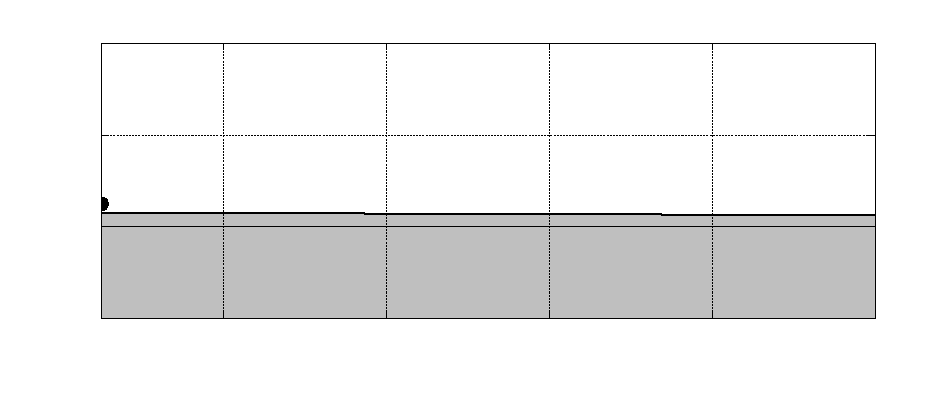
\includegraphics{./Analytic000}}%
    \gplfronttext
  \end{picture}%
\endgroup

  \caption{$\tau = -1$}
 \end{subfigure} \\
 \begin{subfigure}{\textwidth}
  % GNUPLOT: LaTeX picture with Postscript
\begingroup
  \makeatletter
  \providecommand\color[2][]{%
    \GenericError{(gnuplot) \space\space\space\@spaces}{%
      Package color not loaded in conjunction with
      terminal option `colourtext'%
    }{See the gnuplot documentation for explanation.%
    }{Either use 'blacktext' in gnuplot or load the package
      color.sty in LaTeX.}%
    \renewcommand\color[2][]{}%
  }%
  \providecommand\includegraphics[2][]{%
    \GenericError{(gnuplot) \space\space\space\@spaces}{%
      Package graphicx or graphics not loaded%
    }{See the gnuplot documentation for explanation.%
    }{The gnuplot epslatex terminal needs graphicx.sty or graphics.sty.}%
    \renewcommand\includegraphics[2][]{}%
  }%
  \providecommand\rotatebox[2]{#2}%
  \@ifundefined{ifGPcolor}{%
    \newif\ifGPcolor
    \GPcolortrue
  }{}%
  \@ifundefined{ifGPblacktext}{%
    \newif\ifGPblacktext
    \GPblacktexttrue
  }{}%
  % define a \g@addto@macro without @ in the name:
  \let\gplgaddtomacro\g@addto@macro
  % define empty templates for all commands taking text:
  \gdef\gplbacktext{}%
  \gdef\gplfronttext{}%
  \makeatother
  \ifGPblacktext
    % no textcolor at all
    \def\colorrgb#1{}%
    \def\colorgray#1{}%
  \else
    % gray or color?
    \ifGPcolor
      \def\colorrgb#1{\color[rgb]{#1}}%
      \def\colorgray#1{\color[gray]{#1}}%
      \expandafter\def\csname LTw\endcsname{\color{white}}%
      \expandafter\def\csname LTb\endcsname{\color{black}}%
      \expandafter\def\csname LTa\endcsname{\color{black}}%
      \expandafter\def\csname LT0\endcsname{\color[rgb]{1,0,0}}%
      \expandafter\def\csname LT1\endcsname{\color[rgb]{0,1,0}}%
      \expandafter\def\csname LT2\endcsname{\color[rgb]{0,0,1}}%
      \expandafter\def\csname LT3\endcsname{\color[rgb]{1,0,1}}%
      \expandafter\def\csname LT4\endcsname{\color[rgb]{0,1,1}}%
      \expandafter\def\csname LT5\endcsname{\color[rgb]{1,1,0}}%
      \expandafter\def\csname LT6\endcsname{\color[rgb]{0,0,0}}%
      \expandafter\def\csname LT7\endcsname{\color[rgb]{1,0.3,0}}%
      \expandafter\def\csname LT8\endcsname{\color[rgb]{0.5,0.5,0.5}}%
    \else
      % gray
      \def\colorrgb#1{\color{black}}%
      \def\colorgray#1{\color[gray]{#1}}%
      \expandafter\def\csname LTw\endcsname{\color{white}}%
      \expandafter\def\csname LTb\endcsname{\color{black}}%
      \expandafter\def\csname LTa\endcsname{\color{black}}%
      \expandafter\def\csname LT0\endcsname{\color{black}}%
      \expandafter\def\csname LT1\endcsname{\color{black}}%
      \expandafter\def\csname LT2\endcsname{\color{black}}%
      \expandafter\def\csname LT3\endcsname{\color{black}}%
      \expandafter\def\csname LT4\endcsname{\color{black}}%
      \expandafter\def\csname LT5\endcsname{\color{black}}%
      \expandafter\def\csname LT6\endcsname{\color{black}}%
      \expandafter\def\csname LT7\endcsname{\color{black}}%
      \expandafter\def\csname LT8\endcsname{\color{black}}%
    \fi
  \fi
    \setlength{\unitlength}{0.0500bp}%
    \ifx\gptboxheight\undefined%
      \newlength{\gptboxheight}%
      \newlength{\gptboxwidth}%
      \newsavebox{\gptboxtext}%
    \fi%
    \setlength{\fboxrule}{0.5pt}%
    \setlength{\fboxsep}{1pt}%
\begin{picture}(8640.00,3600.00)%
    \gplgaddtomacro\gplbacktext{%
    }%
    \gplgaddtomacro\gplfronttext{%
      \csname LTb\endcsname%
      \put(176,2019){\makebox(0,0){\strut{}$\eta \cdot \frac{v^2}{Gm}$}}%
      \put(4528,154){\makebox(0,0){\strut{}$r \cdot \frac{g}{v^2}$}}%
      \csname LTb\endcsname%
      \put(682,704){\makebox(0,0)[r]{\strut{}$-4$}}%
      \csname LTb\endcsname%
      \put(682,1581){\makebox(0,0)[r]{\strut{}$0$}}%
      \csname LTb\endcsname%
      \put(682,2458){\makebox(0,0)[r]{\strut{}$4$}}%
      \csname LTb\endcsname%
      \put(682,3335){\makebox(0,0)[r]{\strut{}$8$}}%
      \csname LTb\endcsname%
      \put(1987,484){\makebox(0,0){\strut{}$0.2$}}%
      \csname LTb\endcsname%
      \put(3551,484){\makebox(0,0){\strut{}$0.4$}}%
      \csname LTb\endcsname%
      \put(5115,484){\makebox(0,0){\strut{}$0.6$}}%
      \csname LTb\endcsname%
      \put(6679,484){\makebox(0,0){\strut{}$0.8$}}%
      \csname LTb\endcsname%
      \put(8243,484){\makebox(0,0){\strut{}$1$}}%
    }%
    \gplbacktext
    \put(0,0){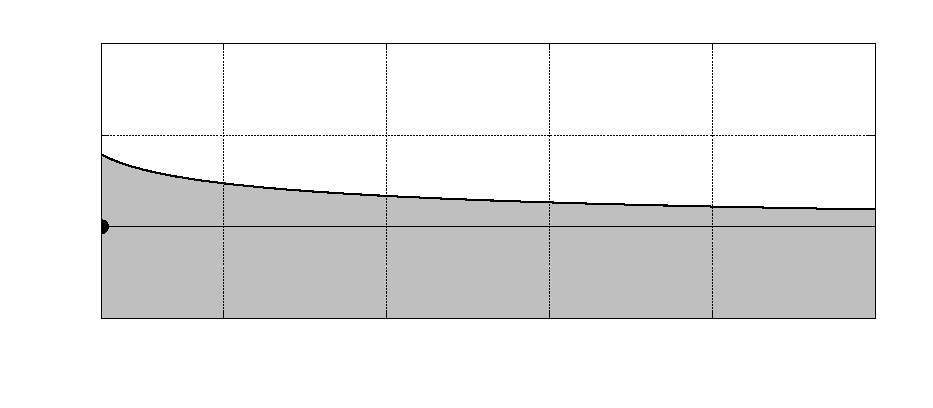
\includegraphics{./Analytic001}}%
    \gplfronttext
  \end{picture}%
\endgroup

  \caption{$\tau = 0$}
 \end{subfigure} \\
 \begin{subfigure}{\textwidth}
  % GNUPLOT: LaTeX picture with Postscript
\begingroup
  \makeatletter
  \providecommand\color[2][]{%
    \GenericError{(gnuplot) \space\space\space\@spaces}{%
      Package color not loaded in conjunction with
      terminal option `colourtext'%
    }{See the gnuplot documentation for explanation.%
    }{Either use 'blacktext' in gnuplot or load the package
      color.sty in LaTeX.}%
    \renewcommand\color[2][]{}%
  }%
  \providecommand\includegraphics[2][]{%
    \GenericError{(gnuplot) \space\space\space\@spaces}{%
      Package graphicx or graphics not loaded%
    }{See the gnuplot documentation for explanation.%
    }{The gnuplot epslatex terminal needs graphicx.sty or graphics.sty.}%
    \renewcommand\includegraphics[2][]{}%
  }%
  \providecommand\rotatebox[2]{#2}%
  \@ifundefined{ifGPcolor}{%
    \newif\ifGPcolor
    \GPcolortrue
  }{}%
  \@ifundefined{ifGPblacktext}{%
    \newif\ifGPblacktext
    \GPblacktexttrue
  }{}%
  % define a \g@addto@macro without @ in the name:
  \let\gplgaddtomacro\g@addto@macro
  % define empty templates for all commands taking text:
  \gdef\gplbacktext{}%
  \gdef\gplfronttext{}%
  \makeatother
  \ifGPblacktext
    % no textcolor at all
    \def\colorrgb#1{}%
    \def\colorgray#1{}%
  \else
    % gray or color?
    \ifGPcolor
      \def\colorrgb#1{\color[rgb]{#1}}%
      \def\colorgray#1{\color[gray]{#1}}%
      \expandafter\def\csname LTw\endcsname{\color{white}}%
      \expandafter\def\csname LTb\endcsname{\color{black}}%
      \expandafter\def\csname LTa\endcsname{\color{black}}%
      \expandafter\def\csname LT0\endcsname{\color[rgb]{1,0,0}}%
      \expandafter\def\csname LT1\endcsname{\color[rgb]{0,1,0}}%
      \expandafter\def\csname LT2\endcsname{\color[rgb]{0,0,1}}%
      \expandafter\def\csname LT3\endcsname{\color[rgb]{1,0,1}}%
      \expandafter\def\csname LT4\endcsname{\color[rgb]{0,1,1}}%
      \expandafter\def\csname LT5\endcsname{\color[rgb]{1,1,0}}%
      \expandafter\def\csname LT6\endcsname{\color[rgb]{0,0,0}}%
      \expandafter\def\csname LT7\endcsname{\color[rgb]{1,0.3,0}}%
      \expandafter\def\csname LT8\endcsname{\color[rgb]{0.5,0.5,0.5}}%
    \else
      % gray
      \def\colorrgb#1{\color{black}}%
      \def\colorgray#1{\color[gray]{#1}}%
      \expandafter\def\csname LTw\endcsname{\color{white}}%
      \expandafter\def\csname LTb\endcsname{\color{black}}%
      \expandafter\def\csname LTa\endcsname{\color{black}}%
      \expandafter\def\csname LT0\endcsname{\color{black}}%
      \expandafter\def\csname LT1\endcsname{\color{black}}%
      \expandafter\def\csname LT2\endcsname{\color{black}}%
      \expandafter\def\csname LT3\endcsname{\color{black}}%
      \expandafter\def\csname LT4\endcsname{\color{black}}%
      \expandafter\def\csname LT5\endcsname{\color{black}}%
      \expandafter\def\csname LT6\endcsname{\color{black}}%
      \expandafter\def\csname LT7\endcsname{\color{black}}%
      \expandafter\def\csname LT8\endcsname{\color{black}}%
    \fi
  \fi
    \setlength{\unitlength}{0.0500bp}%
    \ifx\gptboxheight\undefined%
      \newlength{\gptboxheight}%
      \newlength{\gptboxwidth}%
      \newsavebox{\gptboxtext}%
    \fi%
    \setlength{\fboxrule}{0.5pt}%
    \setlength{\fboxsep}{1pt}%
\begin{picture}(8640.00,3600.00)%
    \gplgaddtomacro\gplbacktext{%
    }%
    \gplgaddtomacro\gplfronttext{%
      \csname LTb\endcsname%
      \put(176,2019){\makebox(0,0){\strut{}$\eta \cdot \frac{v^2}{Gm}$}}%
      \put(4528,154){\makebox(0,0){\strut{}$r \cdot \frac{g}{v^2}$}}%
      \csname LTb\endcsname%
      \put(682,704){\makebox(0,0)[r]{\strut{}$-4$}}%
      \csname LTb\endcsname%
      \put(682,1581){\makebox(0,0)[r]{\strut{}$0$}}%
      \csname LTb\endcsname%
      \put(682,2458){\makebox(0,0)[r]{\strut{}$4$}}%
      \csname LTb\endcsname%
      \put(682,3335){\makebox(0,0)[r]{\strut{}$8$}}%
      \csname LTb\endcsname%
      \put(1987,484){\makebox(0,0){\strut{}$0.2$}}%
      \csname LTb\endcsname%
      \put(3551,484){\makebox(0,0){\strut{}$0.4$}}%
      \csname LTb\endcsname%
      \put(5115,484){\makebox(0,0){\strut{}$0.6$}}%
      \csname LTb\endcsname%
      \put(6679,484){\makebox(0,0){\strut{}$0.8$}}%
      \csname LTb\endcsname%
      \put(8243,484){\makebox(0,0){\strut{}$1$}}%
    }%
    \gplbacktext
    \put(0,0){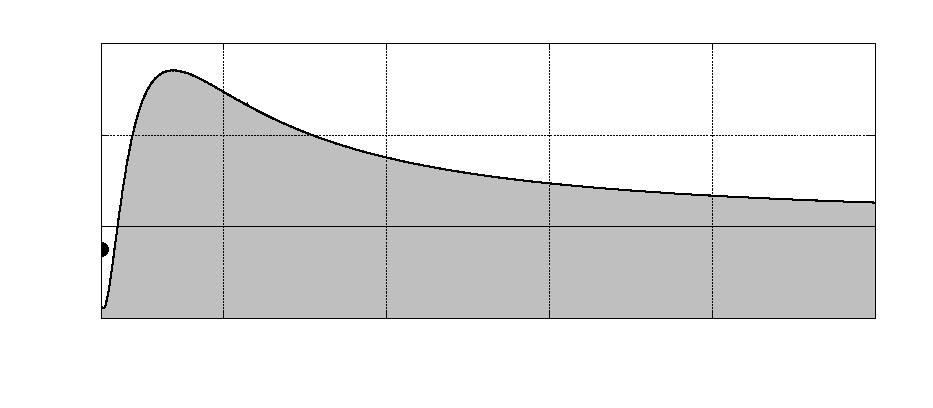
\includegraphics{./Analytic002}}%
    \gplfronttext
  \end{picture}%
\endgroup

  \caption{$\tau = 1$}
 \end{subfigure}
\end{centering}
\end{figure}

\begin{figure}[p] \ContinuedFloat
\begin{centering}
 \begin{subfigure}{\textwidth}
  % GNUPLOT: LaTeX picture with Postscript
\begingroup
  \makeatletter
  \providecommand\color[2][]{%
    \GenericError{(gnuplot) \space\space\space\@spaces}{%
      Package color not loaded in conjunction with
      terminal option `colourtext'%
    }{See the gnuplot documentation for explanation.%
    }{Either use 'blacktext' in gnuplot or load the package
      color.sty in LaTeX.}%
    \renewcommand\color[2][]{}%
  }%
  \providecommand\includegraphics[2][]{%
    \GenericError{(gnuplot) \space\space\space\@spaces}{%
      Package graphicx or graphics not loaded%
    }{See the gnuplot documentation for explanation.%
    }{The gnuplot epslatex terminal needs graphicx.sty or graphics.sty.}%
    \renewcommand\includegraphics[2][]{}%
  }%
  \providecommand\rotatebox[2]{#2}%
  \@ifundefined{ifGPcolor}{%
    \newif\ifGPcolor
    \GPcolortrue
  }{}%
  \@ifundefined{ifGPblacktext}{%
    \newif\ifGPblacktext
    \GPblacktexttrue
  }{}%
  % define a \g@addto@macro without @ in the name:
  \let\gplgaddtomacro\g@addto@macro
  % define empty templates for all commands taking text:
  \gdef\gplbacktext{}%
  \gdef\gplfronttext{}%
  \makeatother
  \ifGPblacktext
    % no textcolor at all
    \def\colorrgb#1{}%
    \def\colorgray#1{}%
  \else
    % gray or color?
    \ifGPcolor
      \def\colorrgb#1{\color[rgb]{#1}}%
      \def\colorgray#1{\color[gray]{#1}}%
      \expandafter\def\csname LTw\endcsname{\color{white}}%
      \expandafter\def\csname LTb\endcsname{\color{black}}%
      \expandafter\def\csname LTa\endcsname{\color{black}}%
      \expandafter\def\csname LT0\endcsname{\color[rgb]{1,0,0}}%
      \expandafter\def\csname LT1\endcsname{\color[rgb]{0,1,0}}%
      \expandafter\def\csname LT2\endcsname{\color[rgb]{0,0,1}}%
      \expandafter\def\csname LT3\endcsname{\color[rgb]{1,0,1}}%
      \expandafter\def\csname LT4\endcsname{\color[rgb]{0,1,1}}%
      \expandafter\def\csname LT5\endcsname{\color[rgb]{1,1,0}}%
      \expandafter\def\csname LT6\endcsname{\color[rgb]{0,0,0}}%
      \expandafter\def\csname LT7\endcsname{\color[rgb]{1,0.3,0}}%
      \expandafter\def\csname LT8\endcsname{\color[rgb]{0.5,0.5,0.5}}%
    \else
      % gray
      \def\colorrgb#1{\color{black}}%
      \def\colorgray#1{\color[gray]{#1}}%
      \expandafter\def\csname LTw\endcsname{\color{white}}%
      \expandafter\def\csname LTb\endcsname{\color{black}}%
      \expandafter\def\csname LTa\endcsname{\color{black}}%
      \expandafter\def\csname LT0\endcsname{\color{black}}%
      \expandafter\def\csname LT1\endcsname{\color{black}}%
      \expandafter\def\csname LT2\endcsname{\color{black}}%
      \expandafter\def\csname LT3\endcsname{\color{black}}%
      \expandafter\def\csname LT4\endcsname{\color{black}}%
      \expandafter\def\csname LT5\endcsname{\color{black}}%
      \expandafter\def\csname LT6\endcsname{\color{black}}%
      \expandafter\def\csname LT7\endcsname{\color{black}}%
      \expandafter\def\csname LT8\endcsname{\color{black}}%
    \fi
  \fi
    \setlength{\unitlength}{0.0500bp}%
    \ifx\gptboxheight\undefined%
      \newlength{\gptboxheight}%
      \newlength{\gptboxwidth}%
      \newsavebox{\gptboxtext}%
    \fi%
    \setlength{\fboxrule}{0.5pt}%
    \setlength{\fboxsep}{1pt}%
\begin{picture}(8640.00,3600.00)%
    \gplgaddtomacro\gplbacktext{%
    }%
    \gplgaddtomacro\gplfronttext{%
      \csname LTb\endcsname%
      \put(176,2019){\makebox(0,0){\strut{}$\frac{\eta}{Gm/v^2}$}}%
      \put(4528,154){\makebox(0,0){\strut{}$\chi$}}%
      \csname LTb\endcsname%
      \put(682,704){\makebox(0,0)[r]{\strut{}$-4$}}%
      \csname LTb\endcsname%
      \put(682,1581){\makebox(0,0)[r]{\strut{}$0$}}%
      \csname LTb\endcsname%
      \put(682,2458){\makebox(0,0)[r]{\strut{}$4$}}%
      \csname LTb\endcsname%
      \put(682,3335){\makebox(0,0)[r]{\strut{}$8$}}%
      \csname LTb\endcsname%
      \put(1987,484){\makebox(0,0){\strut{}$0.2$}}%
      \csname LTb\endcsname%
      \put(3551,484){\makebox(0,0){\strut{}$0.4$}}%
      \csname LTb\endcsname%
      \put(5115,484){\makebox(0,0){\strut{}$0.6$}}%
      \csname LTb\endcsname%
      \put(6679,484){\makebox(0,0){\strut{}$0.8$}}%
      \csname LTb\endcsname%
      \put(8243,484){\makebox(0,0){\strut{}$1$}}%
    }%
    \gplbacktext
    \put(0,0){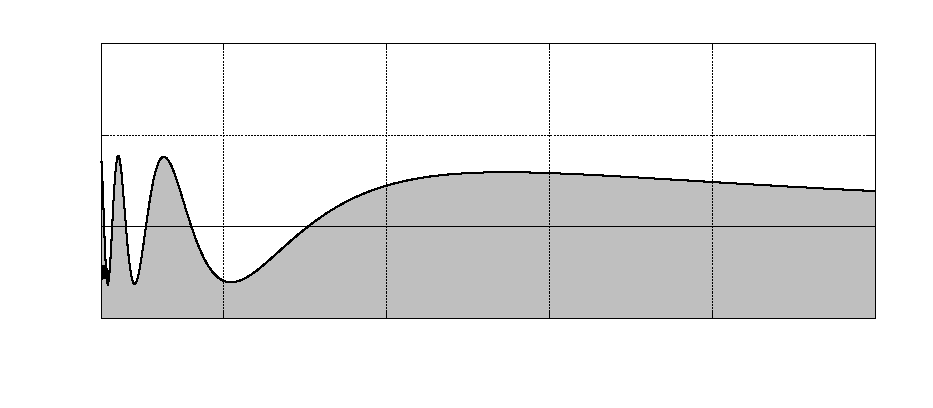
\includegraphics{./3Analytic/Analytic003}}%
    \gplfronttext
  \end{picture}%
\endgroup

  \caption{$\tau = 2$}
 \end{subfigure} \\
 \begin{subfigure}{\textwidth}
  % GNUPLOT: LaTeX picture with Postscript
\begingroup
  \makeatletter
  \providecommand\color[2][]{%
    \GenericError{(gnuplot) \space\space\space\@spaces}{%
      Package color not loaded in conjunction with
      terminal option `colourtext'%
    }{See the gnuplot documentation for explanation.%
    }{Either use 'blacktext' in gnuplot or load the package
      color.sty in LaTeX.}%
    \renewcommand\color[2][]{}%
  }%
  \providecommand\includegraphics[2][]{%
    \GenericError{(gnuplot) \space\space\space\@spaces}{%
      Package graphicx or graphics not loaded%
    }{See the gnuplot documentation for explanation.%
    }{The gnuplot epslatex terminal needs graphicx.sty or graphics.sty.}%
    \renewcommand\includegraphics[2][]{}%
  }%
  \providecommand\rotatebox[2]{#2}%
  \@ifundefined{ifGPcolor}{%
    \newif\ifGPcolor
    \GPcolortrue
  }{}%
  \@ifundefined{ifGPblacktext}{%
    \newif\ifGPblacktext
    \GPblacktexttrue
  }{}%
  % define a \g@addto@macro without @ in the name:
  \let\gplgaddtomacro\g@addto@macro
  % define empty templates for all commands taking text:
  \gdef\gplbacktext{}%
  \gdef\gplfronttext{}%
  \makeatother
  \ifGPblacktext
    % no textcolor at all
    \def\colorrgb#1{}%
    \def\colorgray#1{}%
  \else
    % gray or color?
    \ifGPcolor
      \def\colorrgb#1{\color[rgb]{#1}}%
      \def\colorgray#1{\color[gray]{#1}}%
      \expandafter\def\csname LTw\endcsname{\color{white}}%
      \expandafter\def\csname LTb\endcsname{\color{black}}%
      \expandafter\def\csname LTa\endcsname{\color{black}}%
      \expandafter\def\csname LT0\endcsname{\color[rgb]{1,0,0}}%
      \expandafter\def\csname LT1\endcsname{\color[rgb]{0,1,0}}%
      \expandafter\def\csname LT2\endcsname{\color[rgb]{0,0,1}}%
      \expandafter\def\csname LT3\endcsname{\color[rgb]{1,0,1}}%
      \expandafter\def\csname LT4\endcsname{\color[rgb]{0,1,1}}%
      \expandafter\def\csname LT5\endcsname{\color[rgb]{1,1,0}}%
      \expandafter\def\csname LT6\endcsname{\color[rgb]{0,0,0}}%
      \expandafter\def\csname LT7\endcsname{\color[rgb]{1,0.3,0}}%
      \expandafter\def\csname LT8\endcsname{\color[rgb]{0.5,0.5,0.5}}%
    \else
      % gray
      \def\colorrgb#1{\color{black}}%
      \def\colorgray#1{\color[gray]{#1}}%
      \expandafter\def\csname LTw\endcsname{\color{white}}%
      \expandafter\def\csname LTb\endcsname{\color{black}}%
      \expandafter\def\csname LTa\endcsname{\color{black}}%
      \expandafter\def\csname LT0\endcsname{\color{black}}%
      \expandafter\def\csname LT1\endcsname{\color{black}}%
      \expandafter\def\csname LT2\endcsname{\color{black}}%
      \expandafter\def\csname LT3\endcsname{\color{black}}%
      \expandafter\def\csname LT4\endcsname{\color{black}}%
      \expandafter\def\csname LT5\endcsname{\color{black}}%
      \expandafter\def\csname LT6\endcsname{\color{black}}%
      \expandafter\def\csname LT7\endcsname{\color{black}}%
      \expandafter\def\csname LT8\endcsname{\color{black}}%
    \fi
  \fi
    \setlength{\unitlength}{0.0500bp}%
    \ifx\gptboxheight\undefined%
      \newlength{\gptboxheight}%
      \newlength{\gptboxwidth}%
      \newsavebox{\gptboxtext}%
    \fi%
    \setlength{\fboxrule}{0.5pt}%
    \setlength{\fboxsep}{1pt}%
\begin{picture}(8640.00,3600.00)%
    \gplgaddtomacro\gplbacktext{%
    }%
    \gplgaddtomacro\gplfronttext{%
      \csname LTb\endcsname%
      \put(176,2019){\makebox(0,0){\strut{}$\eta \cdot \frac{v^2}{Gm}$}}%
      \put(4528,154){\makebox(0,0){\strut{}$r \cdot \frac{g}{v^2}$}}%
      \csname LTb\endcsname%
      \put(682,704){\makebox(0,0)[r]{\strut{}$-4$}}%
      \csname LTb\endcsname%
      \put(682,1581){\makebox(0,0)[r]{\strut{}$0$}}%
      \csname LTb\endcsname%
      \put(682,2458){\makebox(0,0)[r]{\strut{}$4$}}%
      \csname LTb\endcsname%
      \put(682,3335){\makebox(0,0)[r]{\strut{}$8$}}%
      \csname LTb\endcsname%
      \put(1987,484){\makebox(0,0){\strut{}$0.2$}}%
      \csname LTb\endcsname%
      \put(3551,484){\makebox(0,0){\strut{}$0.4$}}%
      \csname LTb\endcsname%
      \put(5115,484){\makebox(0,0){\strut{}$0.6$}}%
      \csname LTb\endcsname%
      \put(6679,484){\makebox(0,0){\strut{}$0.8$}}%
      \csname LTb\endcsname%
      \put(8243,484){\makebox(0,0){\strut{}$1$}}%
    }%
    \gplbacktext
    \put(0,0){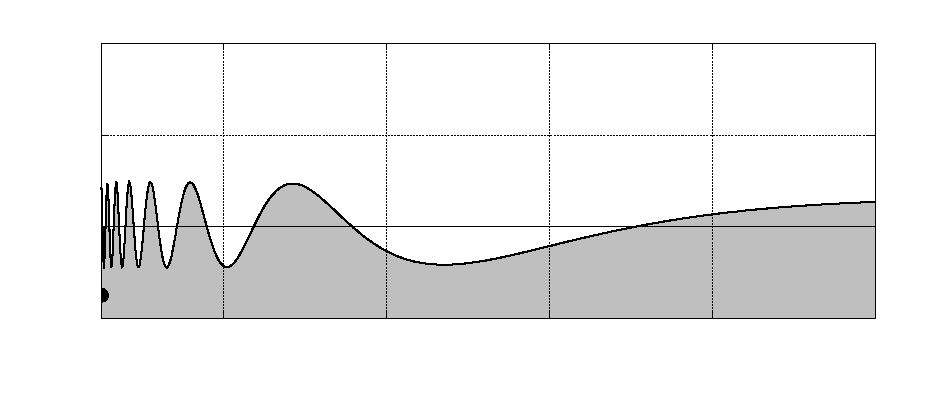
\includegraphics{./Analytic004}}%
    \gplfronttext
  \end{picture}%
\endgroup

  \caption{$\tau = 3$}
 \end{subfigure} \\
  \begin{subfigure}{\textwidth}
  % GNUPLOT: LaTeX picture with Postscript
\begingroup
  \makeatletter
  \providecommand\color[2][]{%
    \GenericError{(gnuplot) \space\space\space\@spaces}{%
      Package color not loaded in conjunction with
      terminal option `colourtext'%
    }{See the gnuplot documentation for explanation.%
    }{Either use 'blacktext' in gnuplot or load the package
      color.sty in LaTeX.}%
    \renewcommand\color[2][]{}%
  }%
  \providecommand\includegraphics[2][]{%
    \GenericError{(gnuplot) \space\space\space\@spaces}{%
      Package graphicx or graphics not loaded%
    }{See the gnuplot documentation for explanation.%
    }{The gnuplot epslatex terminal needs graphicx.sty or graphics.sty.}%
    \renewcommand\includegraphics[2][]{}%
  }%
  \providecommand\rotatebox[2]{#2}%
  \@ifundefined{ifGPcolor}{%
    \newif\ifGPcolor
    \GPcolortrue
  }{}%
  \@ifundefined{ifGPblacktext}{%
    \newif\ifGPblacktext
    \GPblacktexttrue
  }{}%
  % define a \g@addto@macro without @ in the name:
  \let\gplgaddtomacro\g@addto@macro
  % define empty templates for all commands taking text:
  \gdef\gplbacktext{}%
  \gdef\gplfronttext{}%
  \makeatother
  \ifGPblacktext
    % no textcolor at all
    \def\colorrgb#1{}%
    \def\colorgray#1{}%
  \else
    % gray or color?
    \ifGPcolor
      \def\colorrgb#1{\color[rgb]{#1}}%
      \def\colorgray#1{\color[gray]{#1}}%
      \expandafter\def\csname LTw\endcsname{\color{white}}%
      \expandafter\def\csname LTb\endcsname{\color{black}}%
      \expandafter\def\csname LTa\endcsname{\color{black}}%
      \expandafter\def\csname LT0\endcsname{\color[rgb]{1,0,0}}%
      \expandafter\def\csname LT1\endcsname{\color[rgb]{0,1,0}}%
      \expandafter\def\csname LT2\endcsname{\color[rgb]{0,0,1}}%
      \expandafter\def\csname LT3\endcsname{\color[rgb]{1,0,1}}%
      \expandafter\def\csname LT4\endcsname{\color[rgb]{0,1,1}}%
      \expandafter\def\csname LT5\endcsname{\color[rgb]{1,1,0}}%
      \expandafter\def\csname LT6\endcsname{\color[rgb]{0,0,0}}%
      \expandafter\def\csname LT7\endcsname{\color[rgb]{1,0.3,0}}%
      \expandafter\def\csname LT8\endcsname{\color[rgb]{0.5,0.5,0.5}}%
    \else
      % gray
      \def\colorrgb#1{\color{black}}%
      \def\colorgray#1{\color[gray]{#1}}%
      \expandafter\def\csname LTw\endcsname{\color{white}}%
      \expandafter\def\csname LTb\endcsname{\color{black}}%
      \expandafter\def\csname LTa\endcsname{\color{black}}%
      \expandafter\def\csname LT0\endcsname{\color{black}}%
      \expandafter\def\csname LT1\endcsname{\color{black}}%
      \expandafter\def\csname LT2\endcsname{\color{black}}%
      \expandafter\def\csname LT3\endcsname{\color{black}}%
      \expandafter\def\csname LT4\endcsname{\color{black}}%
      \expandafter\def\csname LT5\endcsname{\color{black}}%
      \expandafter\def\csname LT6\endcsname{\color{black}}%
      \expandafter\def\csname LT7\endcsname{\color{black}}%
      \expandafter\def\csname LT8\endcsname{\color{black}}%
    \fi
  \fi
    \setlength{\unitlength}{0.0500bp}%
    \ifx\gptboxheight\undefined%
      \newlength{\gptboxheight}%
      \newlength{\gptboxwidth}%
      \newsavebox{\gptboxtext}%
    \fi%
    \setlength{\fboxrule}{0.5pt}%
    \setlength{\fboxsep}{1pt}%
\begin{picture}(8640.00,3600.00)%
    \gplgaddtomacro\gplbacktext{%
    }%
    \gplgaddtomacro\gplfronttext{%
      \csname LTb\endcsname%
      \put(176,2019){\makebox(0,0){\strut{}$\eta$}}%
      \put(4528,154){\makebox(0,0){\strut{}$r$}}%
      \csname LTb\endcsname%
      \put(682,704){\makebox(0,0)[r]{\strut{}$-4$}}%
      \csname LTb\endcsname%
      \put(682,1581){\makebox(0,0)[r]{\strut{}$0$}}%
      \csname LTb\endcsname%
      \put(682,2458){\makebox(0,0)[r]{\strut{}$4$}}%
      \csname LTb\endcsname%
      \put(682,3335){\makebox(0,0)[r]{\strut{}$8$}}%
      \csname LTb\endcsname%
      \put(1987,484){\makebox(0,0){\strut{}$0.2$}}%
      \csname LTb\endcsname%
      \put(3551,484){\makebox(0,0){\strut{}$0.4$}}%
      \csname LTb\endcsname%
      \put(5115,484){\makebox(0,0){\strut{}$0.6$}}%
      \csname LTb\endcsname%
      \put(6679,484){\makebox(0,0){\strut{}$0.8$}}%
      \csname LTb\endcsname%
      \put(8243,484){\makebox(0,0){\strut{}$1$}}%
    }%
    \gplbacktext
    \put(0,0){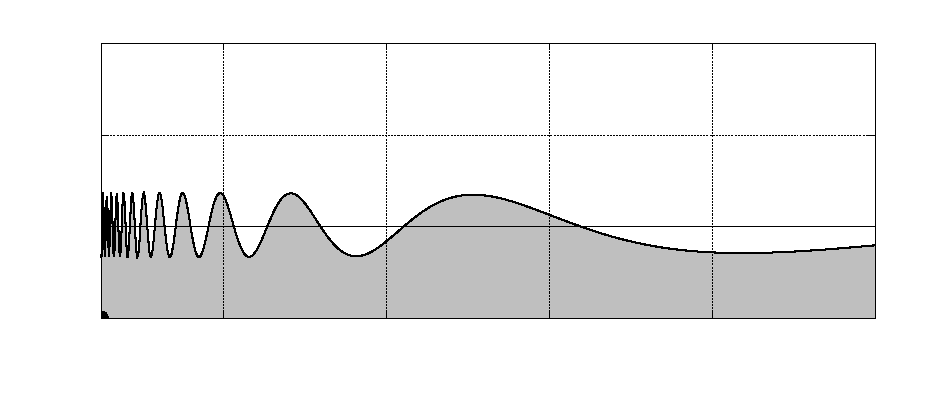
\includegraphics{./Analytic005}}%
    \gplfronttext
  \end{picture}%
\endgroup

  \caption{$\tau = 4$}
 \end{subfigure}
 \end{centering}
 \caption[Analytic Deformation of the Neutron Star]{Deformation of the surface of a neutron star around the time of impact. ***Full animation at .}
 \label{fig:eta}
\end{figure}

This expression for the surface waves can be numerically integrated (the results can be found in Figure \ref{fig:eta}). Initially, before the collision, the primordial black hole causes the surface of the neutron star to rise. At impact, a large wave is created which slowly decays as it traverses outwards. After which waves of smaller and smaller wavelength are observed slowly moving away from the point of impact.

\section{Calculating the Energy Transferred}
\label{chap:energy}

Finally, the last quantity of interest is the energy. Having an idea of what the waves would look like is great, however, if such a collision were to take place, the waves would not be detectable from Earth. On the other hand, the energy would. Now, clearly in order to make reasonable predictions about what would be detected on Earth more than just Newtonian gravity is necessary. Since energy does not escape the system in this model (it is only transferred between the primordial black hole and the neutron star) predictions cannot be made about what such an event would look like from Earth, but it is a worthwhile calculation nonetheless. \\

To calculate the energy transferred we shall start with
\begin{align*}
E(t) &= \frac{1}{2} \rho \int_V \left| \grad \varphi \right|^2 + \rho g \int_V z,
\end{align*}
where $\grad \varphi$ is of course $\overset{\rightharpoonup}u$, which is a typical expression for energy, except we use the density of a fluid element instead of its mass. We can expand the volume integrals out so that 
\begin{align*}
E(t) &= \frac{1}{2} \rho \int_0^{2\pi} \int_0^\infty \int_{-\infty}^0 \left| \grad \varphi \right|^2 \, dz \, r \, dr \, d\theta + \rho g \int_0^{2\pi} \int_0^\infty \int_0^\eta z \, dz \, r \, dr \, d\theta.
\end{align*}
Notice that the bounds on $z$ are from $0$ to $\eta$. This is because we are interested in the change in energy so we subtract the initial potential energy of the neutron star. After solving the trivia integrals we find that
\begin{align*}
E(t) &= \rho \pi \left( \int_0^\infty \int_{-\infty}^0 \left( \frac{\partial \varphi}{\partial r} \right)^2 r \, dz \, dr + \int_0^\infty \int_{-\infty}^0 \left( \frac{\partial \varphi}{\partial z} \right)^2 r \, dz \, dr + g \int_0^\infty \eta^2 r \, dr \right).
\end{align*}
These are non-trivial integrals since $\varphi$, and $\eta$ are themselves non-trivial integrals. To simplify and tidy this calculation, let $\clubsuit$, $\spadesuit$, and $\blacklozenge$ be the three terms respectively, so that $E = \rho \pi (\clubsuit + \spadesuit + g \blacklozenge)$. \\

The reason we wrote the velocity potential, and the deformation of the surface as the Hankel transform of their time components is so these integrals can more easily be solved with the aid of Theorem ***. Starting with the first term,
\begin{align*}
\clubsuit &= \int_0^\infty \int_{-\infty}^0 \left( \frac{\partial \varphi}{\partial r} \right)^2 r \, dz \, dr,
\end{align*}
$\partial \varphi / \partial r$ can be replaced by its Hankel transform representation so that
\begin{align*}
\clubsuit &= \int_{-\infty}^0 \int_0^\infty \Hank[1]{e^{kz}T(t;k)}^2(r,z,t) r \, dr \, dz,
\end{align*}
and after invoking Theorem ***
\begin{align*}
\clubsuit &= \int_{-\infty}^0 \int_0^\infty e^{2kz} T^2(t;k) \, k \, dk \, dz,
\end{align*}
then by integrating over $z$ we get the final expression
\begin{align*}
\clubsuit &= \frac{1}{2} \int_0^\infty T^2(t;k) \, dk.
\end{align*}

Following this same procedure for the other two terms we find that
\begin{align*}
\spadesuit &= \frac{1}{2} \int_0^\infty T^2(t;k) \, dk, \text{ and} \\
\blacklozenge &= \int_0^\infty \frac{\widetilde{T}^2(t;k)}{k} \, dk.
\end{align*}

Combining these we find
\begin{align*}
E(t) = \rho \pi \int_0^\infty T^2(t;k) + g \frac{\widetilde{T}^2(t;k)}{k} \, dk,
\end{align*}
which after expanding out in full
\begin{equation*}
\begin{split}
E(t) = \frac{G^2 m^2 \rho \pi}{g} \int_0^\infty \frac{v^2}{g} \left( \frac{- \sgn(t) e^{-kv |t|} + 2 \Heavi(t) \cos(\omega_k t)}{1+kv^2/g} \right)^2& \\
+ \frac{1}{k} \left( \frac{e^{-kv |t|} + 2 \Heavi(t) v \sqrt{\frac{k}{g}} \sin(\omega_k t)}{1+kv^2/g} \right)^2& \, dk.
\end{split}
\end{equation*}

Using the same substitutions as before, we can nondimensionalize the energy
\begin{equation}
\label{eq:fullenergynon}
\begin{split}
E(\tau) = \frac{G^2 m^2 \rho \pi}{g} \int_0^\infty \left( \frac{- \sgn(\tau) e^{-\kappa |\tau|} + 2 \Heavi(\tau) \cos(\omega_\kappa \tau)}{1+\kappa} \right)^2& \\
+ \left( \frac{e^{-\kappa |\tau|} + 2 \Heavi(\tau) \sqrt{\kappa} \sin(\omega_\kappa \tau)}{1+\kappa} \right)^2& \, dk.
\end{split}
\end{equation}

\begin{figure}[p]
 % GNUPLOT: LaTeX picture with Postscript
\begingroup
  \makeatletter
  \providecommand\color[2][]{%
    \GenericError{(gnuplot) \space\space\space\@spaces}{%
      Package color not loaded in conjunction with
      terminal option `colourtext'%
    }{See the gnuplot documentation for explanation.%
    }{Either use 'blacktext' in gnuplot or load the package
      color.sty in LaTeX.}%
    \renewcommand\color[2][]{}%
  }%
  \providecommand\includegraphics[2][]{%
    \GenericError{(gnuplot) \space\space\space\@spaces}{%
      Package graphicx or graphics not loaded%
    }{See the gnuplot documentation for explanation.%
    }{The gnuplot epslatex terminal needs graphicx.sty or graphics.sty.}%
    \renewcommand\includegraphics[2][]{}%
  }%
  \providecommand\rotatebox[2]{#2}%
  \@ifundefined{ifGPcolor}{%
    \newif\ifGPcolor
    \GPcolortrue
  }{}%
  \@ifundefined{ifGPblacktext}{%
    \newif\ifGPblacktext
    \GPblacktexttrue
  }{}%
  % define a \g@addto@macro without @ in the name:
  \let\gplgaddtomacro\g@addto@macro
  % define empty templates for all commands taking text:
  \gdef\gplbacktext{}%
  \gdef\gplfronttext{}%
  \makeatother
  \ifGPblacktext
    % no textcolor at all
    \def\colorrgb#1{}%
    \def\colorgray#1{}%
  \else
    % gray or color?
    \ifGPcolor
      \def\colorrgb#1{\color[rgb]{#1}}%
      \def\colorgray#1{\color[gray]{#1}}%
      \expandafter\def\csname LTw\endcsname{\color{white}}%
      \expandafter\def\csname LTb\endcsname{\color{black}}%
      \expandafter\def\csname LTa\endcsname{\color{black}}%
      \expandafter\def\csname LT0\endcsname{\color[rgb]{1,0,0}}%
      \expandafter\def\csname LT1\endcsname{\color[rgb]{0,1,0}}%
      \expandafter\def\csname LT2\endcsname{\color[rgb]{0,0,1}}%
      \expandafter\def\csname LT3\endcsname{\color[rgb]{1,0,1}}%
      \expandafter\def\csname LT4\endcsname{\color[rgb]{0,1,1}}%
      \expandafter\def\csname LT5\endcsname{\color[rgb]{1,1,0}}%
      \expandafter\def\csname LT6\endcsname{\color[rgb]{0,0,0}}%
      \expandafter\def\csname LT7\endcsname{\color[rgb]{1,0.3,0}}%
      \expandafter\def\csname LT8\endcsname{\color[rgb]{0.5,0.5,0.5}}%
    \else
      % gray
      \def\colorrgb#1{\color{black}}%
      \def\colorgray#1{\color[gray]{#1}}%
      \expandafter\def\csname LTw\endcsname{\color{white}}%
      \expandafter\def\csname LTb\endcsname{\color{black}}%
      \expandafter\def\csname LTa\endcsname{\color{black}}%
      \expandafter\def\csname LT0\endcsname{\color{black}}%
      \expandafter\def\csname LT1\endcsname{\color{black}}%
      \expandafter\def\csname LT2\endcsname{\color{black}}%
      \expandafter\def\csname LT3\endcsname{\color{black}}%
      \expandafter\def\csname LT4\endcsname{\color{black}}%
      \expandafter\def\csname LT5\endcsname{\color{black}}%
      \expandafter\def\csname LT6\endcsname{\color{black}}%
      \expandafter\def\csname LT7\endcsname{\color{black}}%
      \expandafter\def\csname LT8\endcsname{\color{black}}%
    \fi
  \fi
    \setlength{\unitlength}{0.0500bp}%
    \ifx\gptboxheight\undefined%
      \newlength{\gptboxheight}%
      \newlength{\gptboxwidth}%
      \newsavebox{\gptboxtext}%
    \fi%
    \setlength{\fboxrule}{0.5pt}%
    \setlength{\fboxsep}{1pt}%
\begin{picture}(8640.00,6480.00)%
    \gplgaddtomacro\gplbacktext{%
    }%
    \gplgaddtomacro\gplfronttext{%
      \csname LTb\endcsname%
      \put(176,3459){\rotatebox{-270}{\makebox(0,0){\strut{}$E \cdot \frac{g}{G^2m^2 \rho}$}}}%
      \put(4594,154){\makebox(0,0){\strut{}$t \cdot \frac{g}{v}$}}%
      \csname LTb\endcsname%
      \put(814,1411){\makebox(0,0)[r]{\strut{}$100$}}%
      \csname LTb\endcsname%
      \put(814,2843){\makebox(0,0)[r]{\strut{}$120$}}%
      \csname LTb\endcsname%
      \put(814,4275){\makebox(0,0)[r]{\strut{}$140$}}%
      \csname LTb\endcsname%
      \put(814,5708){\makebox(0,0)[r]{\strut{}$160$}}%
      \csname LTb\endcsname%
      \put(946,484){\makebox(0,0){\strut{}$-30$}}%
      \csname LTb\endcsname%
      \put(2162,484){\makebox(0,0){\strut{}$-20$}}%
      \csname LTb\endcsname%
      \put(3378,484){\makebox(0,0){\strut{}$-10$}}%
      \csname LTb\endcsname%
      \put(4595,484){\makebox(0,0){\strut{}$0$}}%
      \csname LTb\endcsname%
      \put(5811,484){\makebox(0,0){\strut{}$10$}}%
      \csname LTb\endcsname%
      \put(7027,484){\makebox(0,0){\strut{}$20$}}%
      \csname LTb\endcsname%
      \put(8243,484){\makebox(0,0){\strut{}$30$}}%
    }%
    \gplbacktext
    \put(0,0){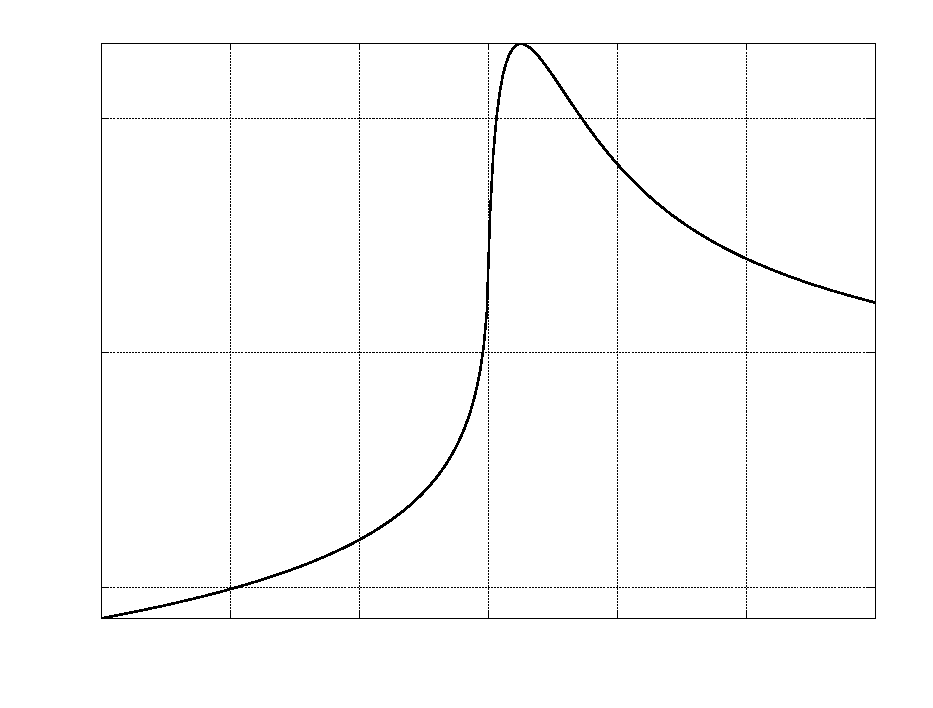
\includegraphics{./AnalyticEnergyPlot}}%
    \gplfronttext
  \end{picture}%
\endgroup

 \caption[Analytic Energy Transfer]{Energy transfer of the interaction for short times; with units of energy of $\frac{G^2 m^2 \rho \pi}{g}$.}
 \label{fig:energy}
\end{figure}

Figure \ref{fig:energy} shows a plot of the energy for times near the collision. Initially, the energy grows exponentially, then at $t=0$, when the primordial black hole collides with the neutron star, a considerable amount of energy is deposited. After which a majority of the energy is carried away exponentially by the primordial black hole. The long time limit is perhaps more useful since that is the net energy transfer of the interaction. By taking the limit as $t \rightarrow \infty$ of \eqref{eq:fullenergynon}, the exponential terms decay to zero, and the sine and cosine simplify to $1$. This new integrand has an elementary antiderivative, and so after integrating, the energy becomes
\begin{align}
\label{eq:energy}
E = 4 \pi \rho \frac{G^2 m^2}{g}
\end{align}
which is a surprisingly compact form. \\

The dynamical friction approach *** finds that the energy loss is
\begin{align*}
E &= \frac{4 G^2 m^2 M}{R^2} \left< \frac{\ln \Lambda}{v^2} \right>,
\end{align*}
where the logarithmic term is the Coulomb logarithm, which in the case of typical stars is approximately $30$. We can compare this to our answer by assuming the average velocity is on the order of the escape velocity
\begin{align*}
\left< v^2 \right> = \frac{2GM}{R},
\end{align*}
and by using the usual form for gravitational acceleration. Then, our expression for the energy can then be simplified to
\begin{align*}
E &= \frac{3Gm^2}{R},
\end{align*}
and the dynamical friction expression to
\begin{align*}
E &= \frac{2Gm^2}{R} \ln \Lambda
\end{align*}
which agrees to within around an order of magnitude.




%\end{document}





















\begin{thebibliography}{}

\bibitem[Navarro, Frenk, \& White(1995)]{nfw95} Navarro, J.F., Frenk, C.S., \& White, S.D.M.  1995, MNRAS, 275, 720

\end{thebibliography}

\appendix

\chapter{A Sample Appendix}
\label{app:sample}

This is just an example of an appendix.

\end{document}